
\documentclass[preprint,12pt]{elsarticle}

\usepackage[spanish]{babel}
\usepackage{amssymb}
\usepackage{graphicx}
\usepackage{lineno}
\usepackage[utf8]{inputenc}
\usepackage{url}
\usepackage{natbib} 
\usepackage{amsmath} 
\usepackage{amssymb} 
\usepackage{float}

\begin{document}
	
	\begin{frontmatter} 

		\title{\huge LABORATORIO 08 - INSTALACION DE UN GESTOR DE BASE DE DATOS ORACLE}
		
		\author{Robles Flores Anthony Richard         	(2016056192)} 
		\address{Escuela Profesional de Ingeniería de Sistemas}
		\address{Universidad Privada de Tacna}
		\address{Tacna, Perú}
		

	\end{frontmatter}



\section{INFORMACIÓN GENERAL} 

\subsection {\textbf{Objetivos}}
\begin{itemize}
	\item Instalar un Gestor de Base de Datos Oracle
\end{itemize}

\subsection {\textbf{Equipos, materiales, programas y recursos utilizados}}
\begin{itemize}
	\item Computadora con sistema operativo Windows 10.
	\item Min 4GB de RAM
	\item Docker Desktop
	\item Oracle SQL Developer
\end{itemize}


\section{Marco Teórico}



\subsection {\textbf{Docker}}
La palabra "DOCKER" se refiere a varias cosas. Esto incluye un proyecto de la comunidad open source; las herramientas del proyecto open source; Docker Inc., la empresa que es la principal promotora de ese proyecto; y las herramientas que la empresa admite formalmente. El hecho de que las tecnologías y la empresa compartan el mismo nombre puede ser confuso.
\subsubsection{\textbf{SQL Server Management Studio}}
SQL Server Management Studio (SSMS) es un entorno integrado para administrar cualquier infraestructura SQL, desde SQL Server hasta Azure SQL Database. SSMS proporciona herramientas para configurar, monitorear y administrar instancias de SQL Server y bases de datos. Use SSMS para implementar, monitorear y actualizar los componentes de nivel de datos utilizados por sus aplicaciones, y crear consultas y scripts.


\section{PROCEDIMIENTO}

\subsubsection{\textbf{Paso 1: Ingresar a Docker Setup}}
\begin{figure}[H]
	\begin{center}
		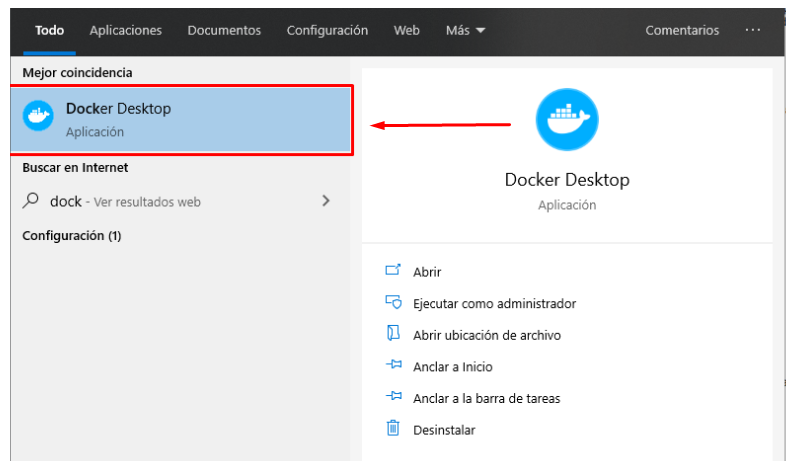
\includegraphics[width=12cm]{./IMAGENES/foto1} 
	\end{center}
\end{figure}

\begin{figure}[H]
	\begin{center}
		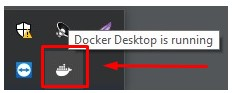
\includegraphics[width=12cm]{./IMAGENES/foto2} 
		\caption{Podremos ver que Docker se encuentra en ejecucion}
	\end{center}
\end{figure}

\begin{figure}[H]
	\begin{center}
		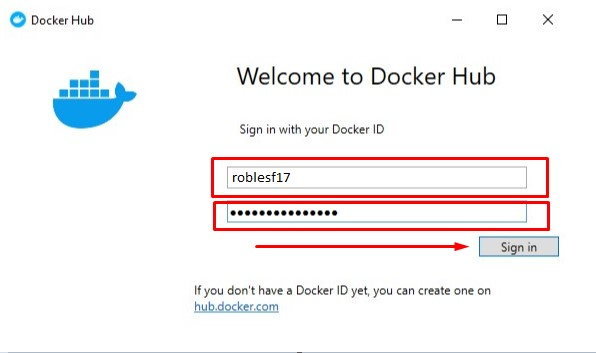
\includegraphics[width=12cm]{./IMAGENES/foto3} 
		\caption{Es necesario ingresar la cuenta Docker}
	\end{center}
\end{figure}

\begin{figure}[H]
	\begin{center}
		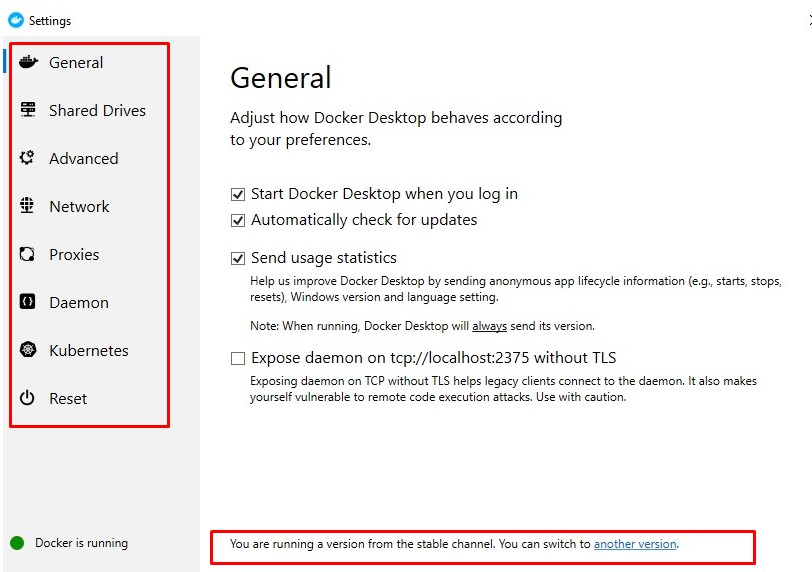
\includegraphics[width=12cm]{./IMAGENES/foto4} 
		\caption{Aqui podemos apreciar la ventana principal de Docker}
	\end{center}
\end{figure}

\subsubsection{\textbf{Paso 2: Utilizaremos PowerShell para gestionar}}

\begin{figure}[H]
	\begin{center}
		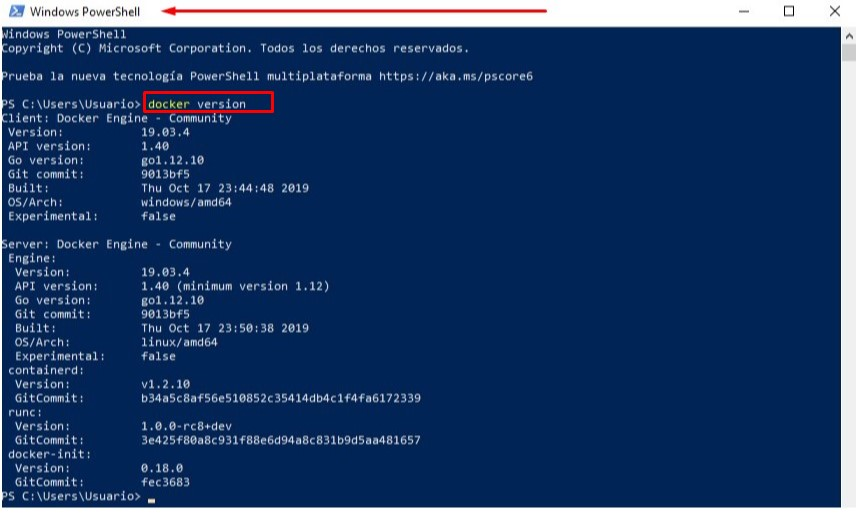
\includegraphics[width=12cm]{./IMAGENES/foto5} 
		\caption{“Docker versión” para confirmar la instalacion de Docker}
	\end{center}
\end{figure}


\begin{figure}[H]
	\begin{center}
		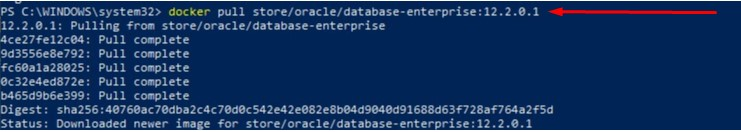
\includegraphics[width=12cm]{./IMAGENES/foto6} 
		\caption{Descargamos la iso}
	\end{center}
\end{figure}

\begin{figure}[H]
	\begin{center}
		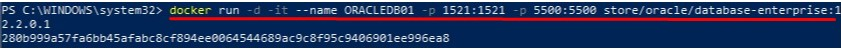
\includegraphics[width=12cm]{./IMAGENES/foto10} 
		\caption{Instalamos el contenedor}
	\end{center}
\end{figure}

\begin{figure}[H]
	\begin{center}
		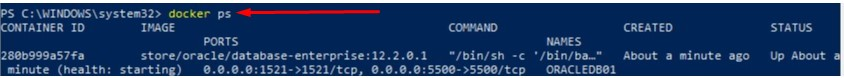
\includegraphics[width=12cm]{./IMAGENES/foto11} 
		\caption{Verificamos se instalo correctamente}
	\end{center}
\end{figure}

\subsubsection{\textbf{Paso 3: Ejecutar}}
\begin{figure}[H]
	\begin{center}
		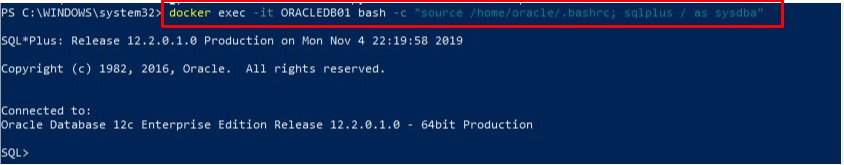
\includegraphics[width=12cm]{./IMAGENES/foto12} 
		\caption{Ejecutaremos el docker}
	\end{center}
\end{figure}

\begin{figure}[H]
	\begin{center}
		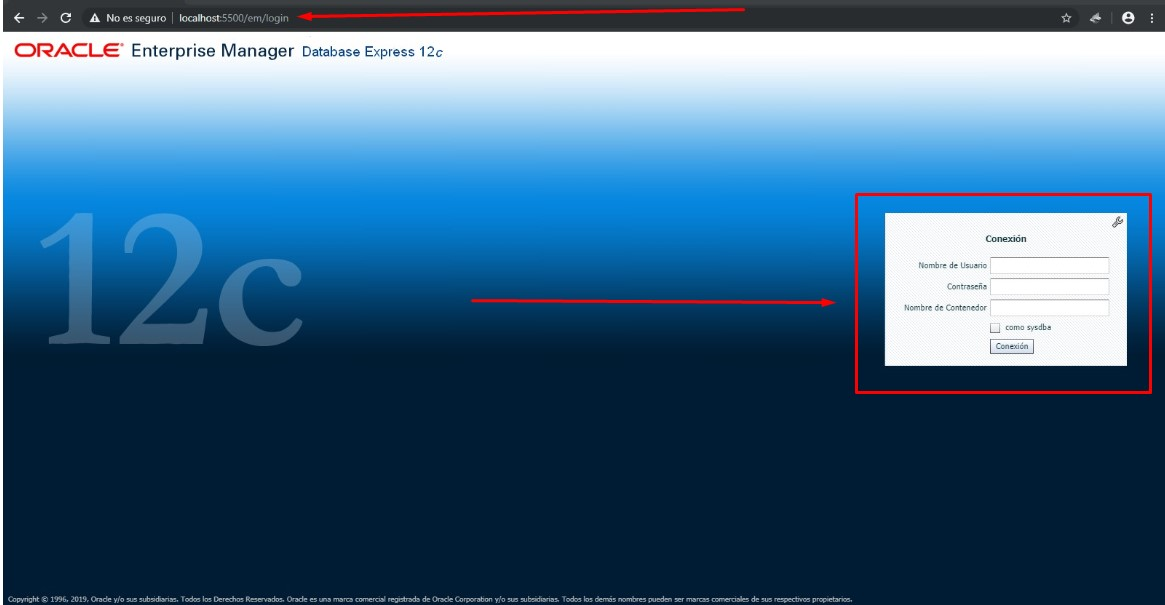
\includegraphics[width=12cm]{./IMAGENES/foto13} 
		\caption{Conectemos a la base de datos creadas}
	\end{center}
\end{figure}

\begin{figure}[H]
	\begin{center}
		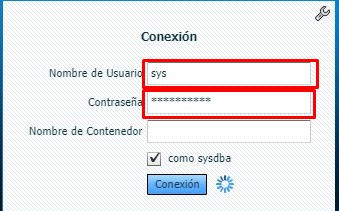
\includegraphics[width=12cm]{./IMAGENES/foto14} 
		\caption{Accederemos de la forma predeterminada}
	\end{center}
\end{figure}

\begin{figure}[H]
	\begin{center}
		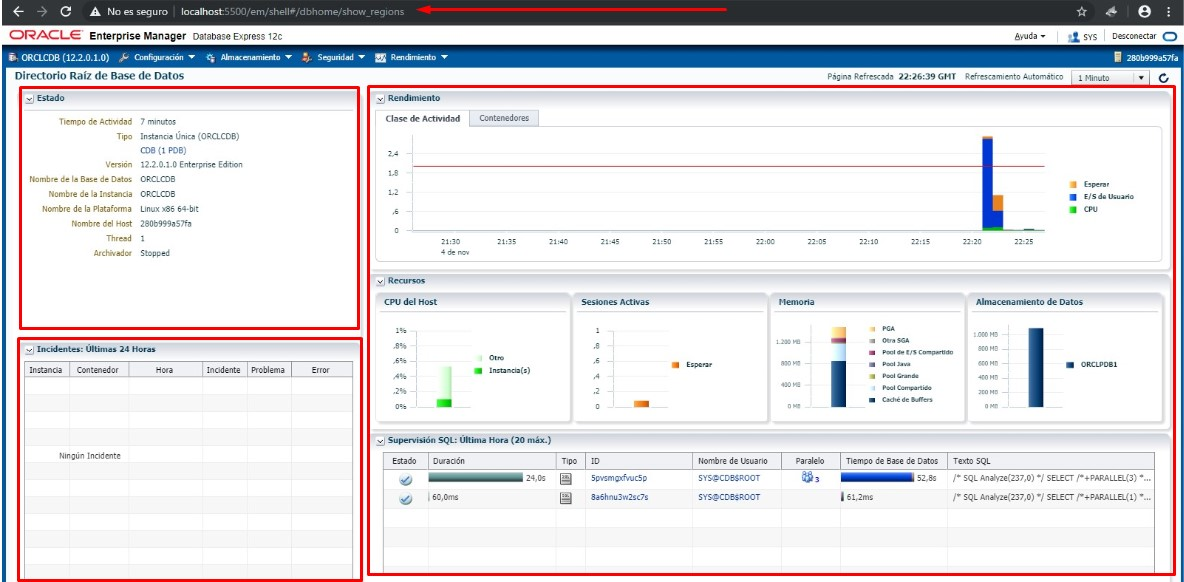
\includegraphics[width=12cm]{./IMAGENES/foto15} 
		\caption{Interfaz grafica principal de ORACLE}
	\end{center}
\end{figure}


\section{ANALISIS E INTERPRETACION DE RESULTADOS }
\begin{itemize}
	\item ¿Qué indican los resultados? \\
	Se reaclizo exitosamente la conexion con el contenedor de base de datos.
	\item ¿Que se ha encontrado?\\
	Tener una base de datos Oracler sin necesidad de estar haciendo toda la instalación necesaria en el computador.
\end{itemize}


\section{CONCLUSION}
Docker es una herramienta de código abierto que desde hace ya algunos años se está hablando mucho y cada vez más. Con Docker podremos ejecutar un conjunto de procesos de forma aislada, crear herramientas gracias a sus imágenes y compartirlas gracias al repositorio que tienen.

\end{document}
